

\subsection{Inducing a Correlation Trap}
\label{sxn:empirical-correlation_trap}

\begin{figure}[t]
    \centering
    \subfigure[MLP3 \LearningRate $16\times$]{
%        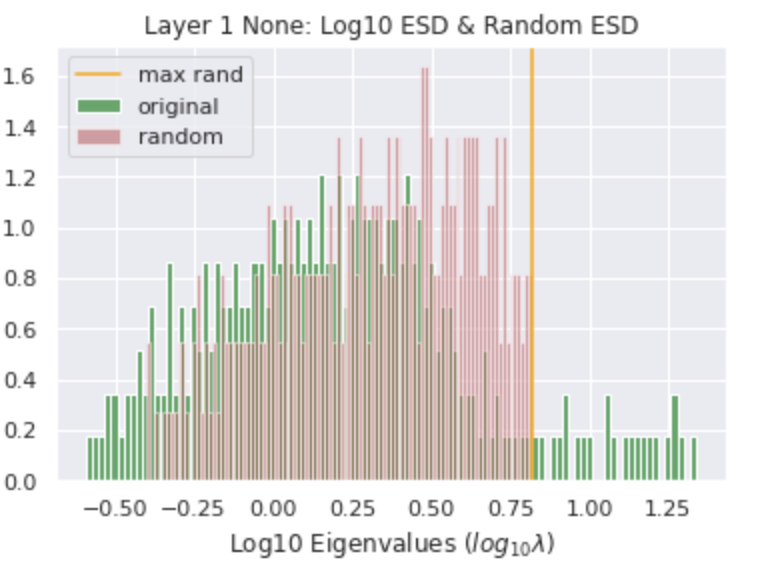
\includegraphics[width=6cm]{img/log-esd-bs2.png}
        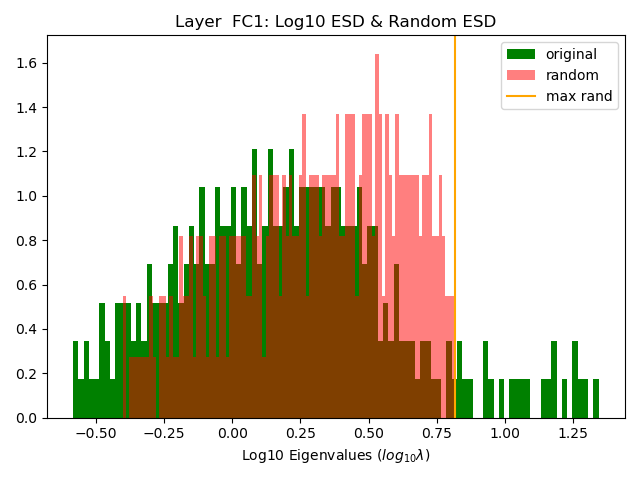
\includegraphics[width=6cm]{img/correlation_traps/LR_16_FC1_0/ww.layer3.randesd2.png}
        \label{fig:mlp3-accuracies3_lr16_trap}
    }
    \subfigure[MLP3 \LearningRate $32\times$]{
        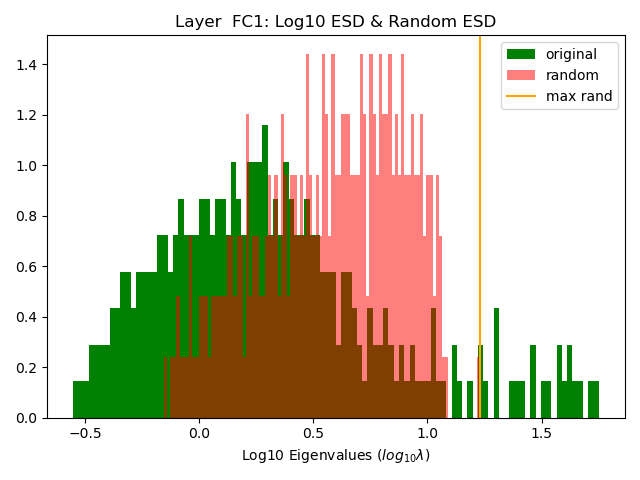
\includegraphics[width=6cm]{img/correlation_traps/LR_32_FC1_0/ww.layer3.randesd2.png}
        \label{fig:mlp3-accuracies3_lr32_trap}
    }
    \caption{ESD plots for learning rate $lr=16\times$ and $lr=32\times$ normal, shown on Log-Lin scale, as computed 
    using the \WW tool, for the FC1 weight matrix $\mathbf{W}$ (green) and an element-wise randomized $\mbox{rand}(\mathbf{W})$ (red).  
    This provides an example of inducing a \CorrelationTrap in the MLP3 model, simply by increasing the learning rate used during model training.  
        See Section~\ref{sxn:Traps}.
            }
    \label{fig:mlp3-accuracies3}
\end{figure}


Previous work on the \HTSR \Phenomenology \cite{MM20a_trends_NatComm,MM21a_simpsons_TR} has shown that one can look for 
quantitative deviations from the necessary pre-conditions of tradtitional \RMT (particularly that the weights are 
$0$-mean and finite variance) to detect when a model layer suffers from some other anomaly in the elements, which we 
call a ``\CorrelationTrap (see Section~\ref{sxn:Traps} and ~\cite{MM20a_trends_NatComm,MM21a_simpsons_TR}). A 
\CorrelationTrap may cause, or be caused by, the over-regularization leading \ALPHA to fall below $2$, (see 
Section~\ref{sxn:underfitting}). Here, we explore this in greater detail, in light of our \SETOL.
% \michael{MOst of this discussion in this par is diff than correlation trap, so we may need to move it elsewhere and update it here.}

% Recall that a \CorrelationTrap arises when the randomized spectrum 
% is not an MP distribution. In this case, we know contrapositively that one or more of the MPs conditions on the 
% element-wise distribution ($0$-mean and finite variance) are not met. When the MP laws conditions are not met, we do 
% not have the usual guarantee that the element-wise distribution alone \emph{cannot} produce a large eigenvalue, meaning 
% that some of the large eigenvalues are likely not a result of correlations between pairs of data elements. 
%
Lets look at the ESDs of the FC1 layer of the MLP3 model, for learning rates $lr=16\times$ and $lr=32\times$ normal. 
We will be interested in the general shape of the ESD of $\tfrac{1}{N}\mathbf{W}^T\mathbf{W}$.
For the purposes of detecting a \CorrelationTrap, we will randomize $\mathbf{W}^T\mathbf{W}$ element-wise, and then observe its largest eigenvalue $\lambda^{max}_{rand}$. 
%%Randomizing element-wise is a way of drawing a sample random matrix whose elements are i.i.d.  from the same distribution as $\mathbf{W}^T\mathbf{W}$, so that any violations of the MP laws preconditions can be seen. 

Figure~\ref{fig:mlp3-accuracies3} shows the ESDs of the original matrix (green) and the element-wise 
randomized $\mbox{rand}(\tfrac{1}{N}\mathbf{W}^T\mathbf{W})$ (red). 
Observe in particular $\lambda^{max}_{rand}$ for each learning rate factor.
For $lr=16\times$, Figure~\ref{fig:mlp3-accuracies3_lr16_trap} shows 
that the ESD of $\tfrac{1}{N}\mathbf{W}^T\mathbf{W}$ is HT, whereas the ESD of the randomized matrix is essentially a distorted semi-circle---as expected from the well-known MP result; and 
that $\lambda^{max}_{rand}$ lies at the edge of the random \MPBulk ESD.
(A similar result is seen for smaller learning rates.)  
In contrast, for $lr=32\times$, Figure~\ref{fig:mlp3-accuracies3_lr32_trap} shows 
that while the original ESD is again HT, the ESD of the randomized has one large element, $\lambda^{max}_{rand}$, that pulls out from the MP bulk.
%
This is the signature of a \CorrelationTrap; and it co-occurrs with the exact learning rate setting that degraded the train and test accuracies, pushing \ALPHA below its optimal value of $\alpha\simeq 2$.
%
When this happens,  both the estimation of \ALPHA and the formation of a PL tail are potentially disrupted. 
%
%%Thus, by increasing the learning rate to $lr=32\times$ normal, we were able to systematically induce a \CorrelationTrap, 

\CorrelationTraps have been observed previously~\cite{MM20a_trends_NatComm,MM21a_simpsons_TR}, using the \HTSR \Phenomenology.
However, \SETOL provides an explanation for why this would be expected to occur --- non-standard element-wise distributions will tend to interfere with the properties of the spectrum which \SETOL analyzes. 
Our derivation in Section~\ref{sxn:empirical} suggests that in order to apply the \SETOL effectively one must avoid (or remove) such traps. 
This too has been observed previously~\cite{MM20a_trends_NatComm,MM21a_simpsons_TR}. 


%\chris{There was some old discussion on alphahat that I have commented here.}
%Notice that, in Figure~\ref{fig:mlp3-accuracies2_mlp3-alphahat},
%and in contrast to \ALPHA, however, the \ALPHAHAT value for $bs=1$ is larger, not smaller,
%and almost follows the trend the other values show.   This happens because
%the \ALPHAHAT metric corrects for the anomalous \Scale in the $bs=1$ case.
%Since $\ALPHAHATEQN=\alpha\log_{10}\lambda_{max}$, the metric multiplies the spuriously
%small $\alpha$ by the spuriously large $\log_{10}\lambda_{max}$, and there
%is a fortuitous cancellation of errors.  This is, in part, why the (layer averaged)
%\ALPHAHAT can describe trends in the quality of models when using just \ALPHA fails.


